\documentclass[dvisvgm,multi=true]{standalone}
\usepackage{mathmlcoresvg}
\begin{document}
% <figcaption><span>Figure 6: </span>Symmetric and non-symmetric stretching of vertical operators</figcaption>
  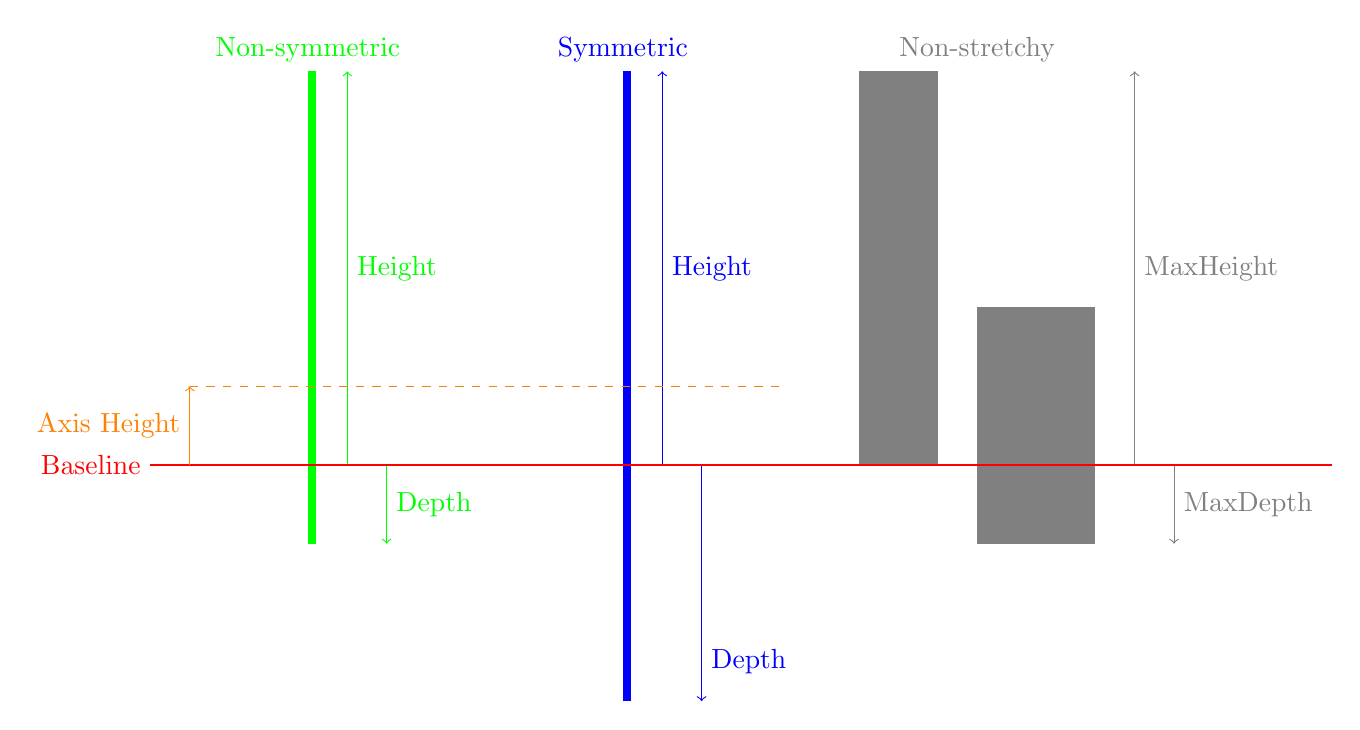
\begin{tikzpicture}[yscale=-1]
  \fill[green](2,-5) node[above]{Non-symmetric} rectangle (2.1,1);
  \draw[green,->](2.5,0) -- (2.5, -2.5) node[right]{Height} -- (2.5,-5);
  \draw[green,->](3,0) -- (3, .5) node[right]{Depth} -- (3,1);

  \fill[blue](6,-5) node[above]{Symmetric} rectangle (6.1,3);
  \draw[blue,->](6.5,0) -- (6.5, -2.5) node[right]{Height} -- (6.5,-5);
  \draw[blue,->](7,0) -- (7, 2.5) node[right]{Depth} -- (7,3);

  \draw[gray](10.5,-5) node[above]{Non-stretchy};
  \fill[gray](9,-5) rectangle (10,0);
  \fill[gray](10.5,-2) rectangle (12,1);
  \draw[gray,->](12.5,0) -- (12.5, -2.5) node[right]{MaxHeight} -- (12.5,-5);
  \draw[gray,->](13,0) -- (13, .5) node[right]{MaxDepth} -- (13,1);

  \draw[red] (0,0) node[left]{Baseline} -- (15,0);
  \draw[->,orange] (.5,0) -- (.5,-.5) node[left]{Axis Height} -- (.5,-1);
  \draw[orange,dashed] (.5,-1) -- (8,-1);
  \end{tikzpicture}

\end{document}
